\documentclass[a4paper,12pt]{article}
\usepackage{graphicx}
\usepackage{caption}
\usepackage{booktabs}
\usepackage{geometry}
\geometry{margin=1in}

\begin{document}

\begin{titlepage}
	\centering

	\huge \textbf{EE 671: VLSI Design} \\
	\vspace{1cm}

	\LARGE \textsc{Assignment 4} \\ \vspace{4.5cm}

	
\includegraphics[width=0.55\textwidth]{../icon.png} \\

	\vspace{4.5cm}

	\Large
	\begin{tabular}{rl}
		\textbf{Student Names:}   & Bhuvansh Goyal (22B3908)   \\
		                          & Saarthak Krishan (22B3959) \\
		                          & Hardik Jangir (22B3901)    \\
		                          & Sambhavi Jaiswal (24D0545) \\
		\textbf{Instructor:}      & Prof. Laxmeesha Somappa    \\
		\textbf{Submission Date:} & 18 Oct 2025
	\end{tabular}

	\vfill
\end{titlepage}

\clearpage

\tableofcontents

\section{Physical Design Violation Checks}

\subsection{DRC Check}
\begin{figure}[htbp!]
	\centering
	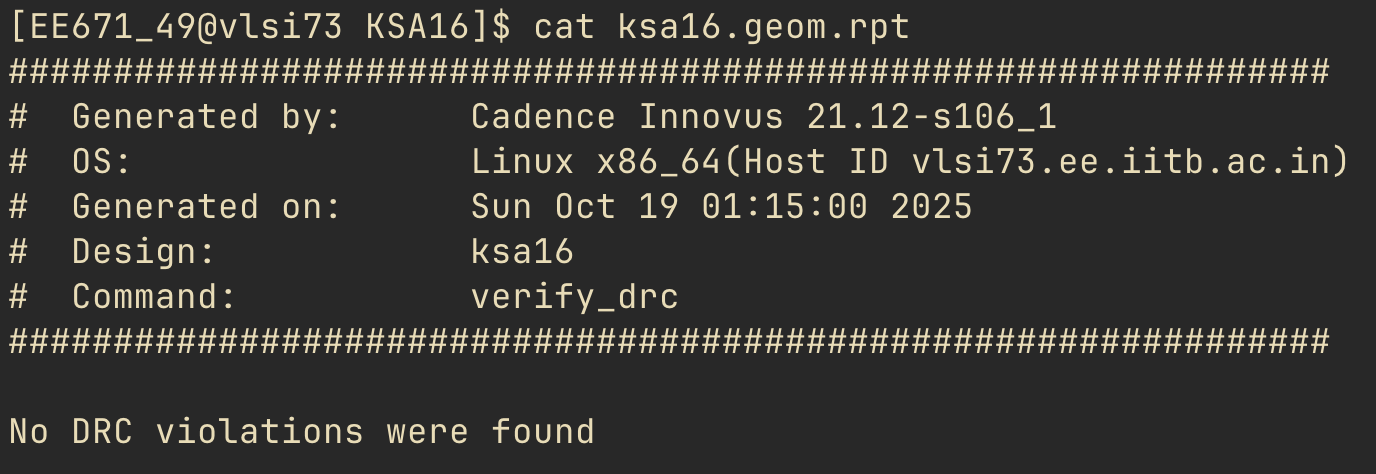
\includegraphics[width=0.95\textwidth]{drc.png}
	\caption{Design Rule Check (DRC) violations overview}
\end{figure}

\subsection{Antenna Check}
\begin{figure}[htbp!]
	\centering
	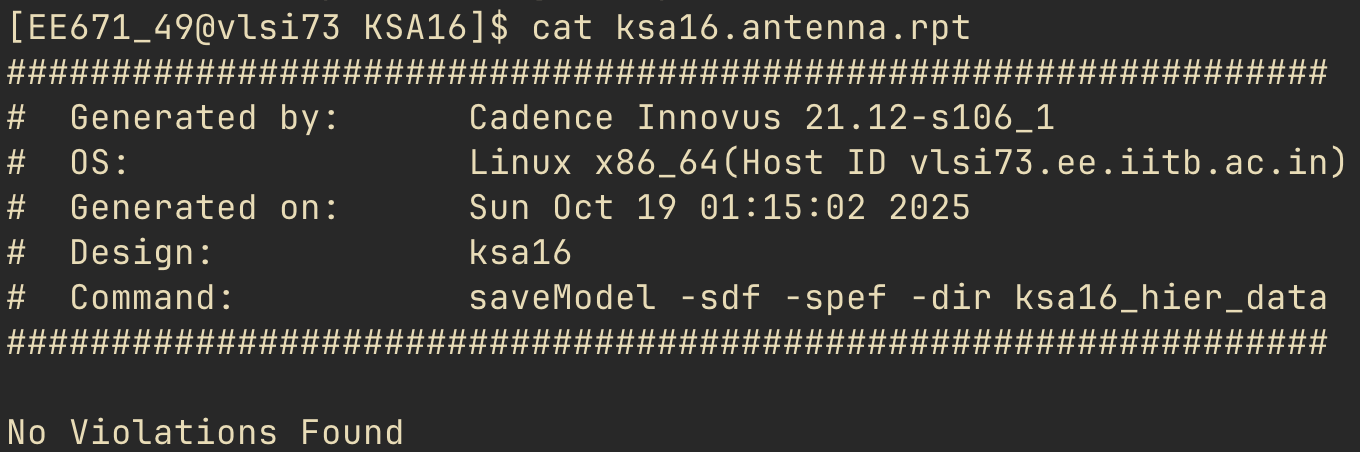
\includegraphics[width=0.95\textwidth]{antenna.png}
	\caption{Antenna check for the layout}
\end{figure}

\subsection{Connectivity Check}

\begin{figure}[htbp!]
	\centering
	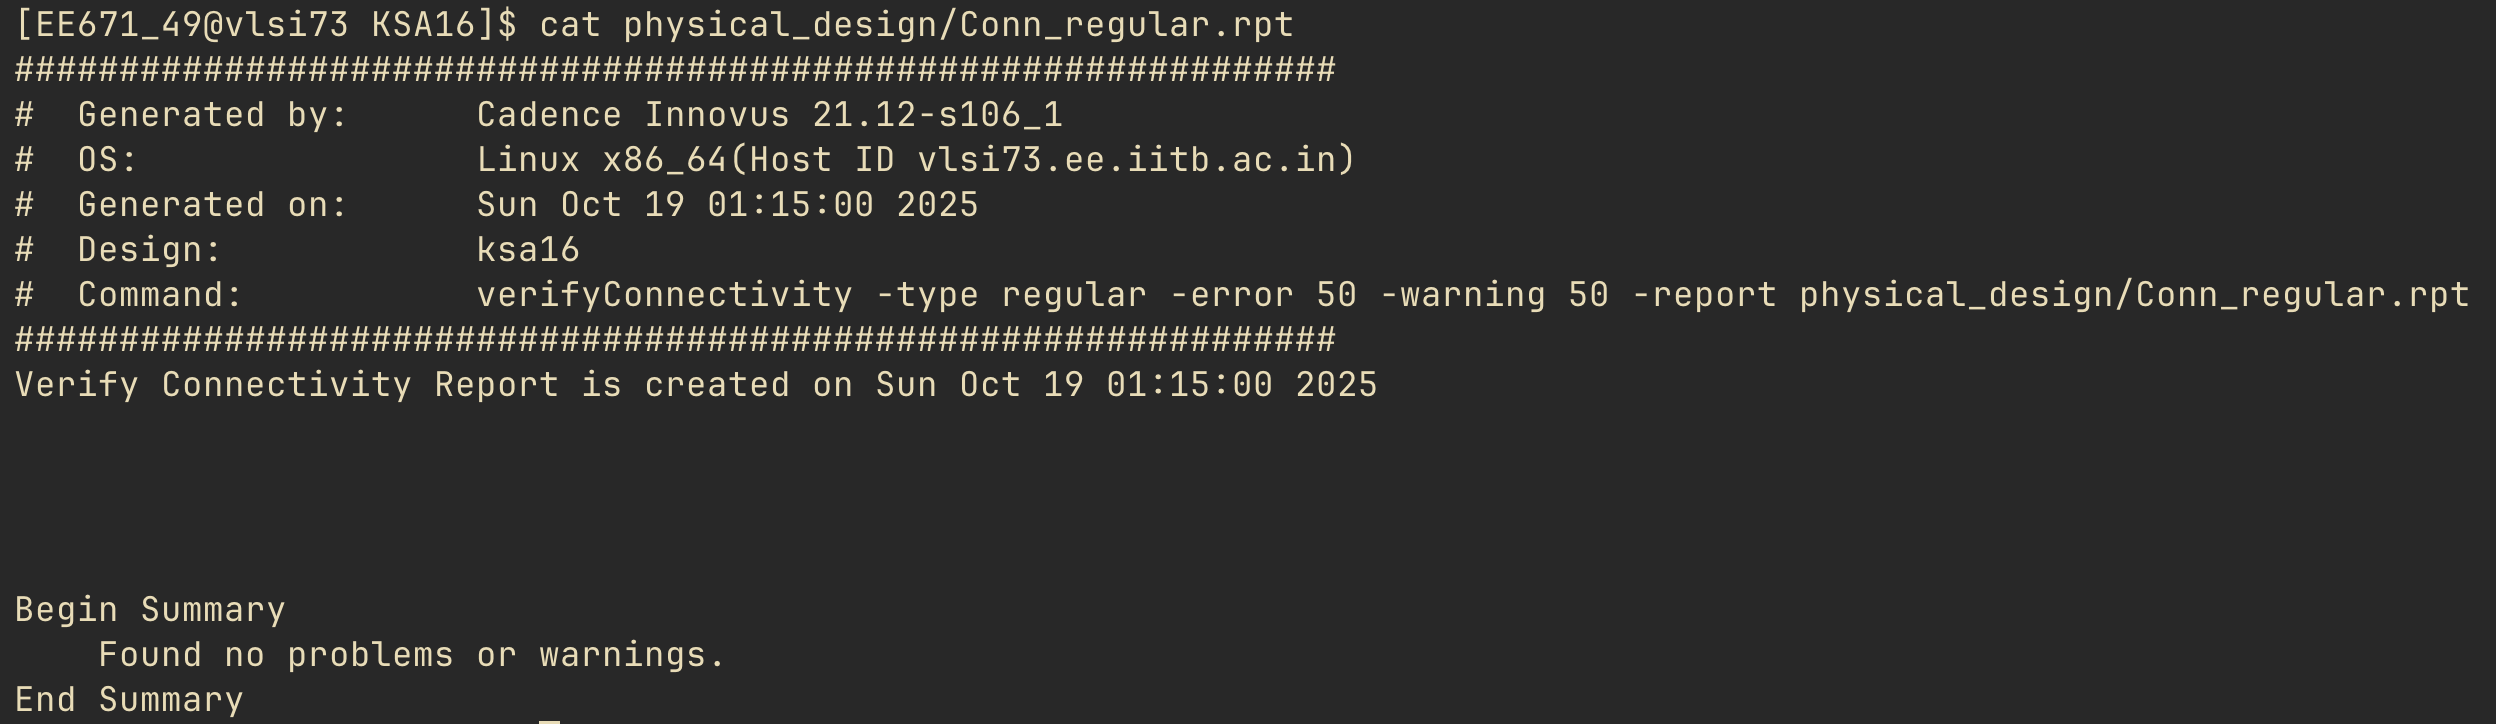
\includegraphics[width=0.95\textwidth]{conn_reg.png}
	\caption{Connectivity check for regular cells}
\end{figure}

\begin{figure}[htbp!]
	\centering
	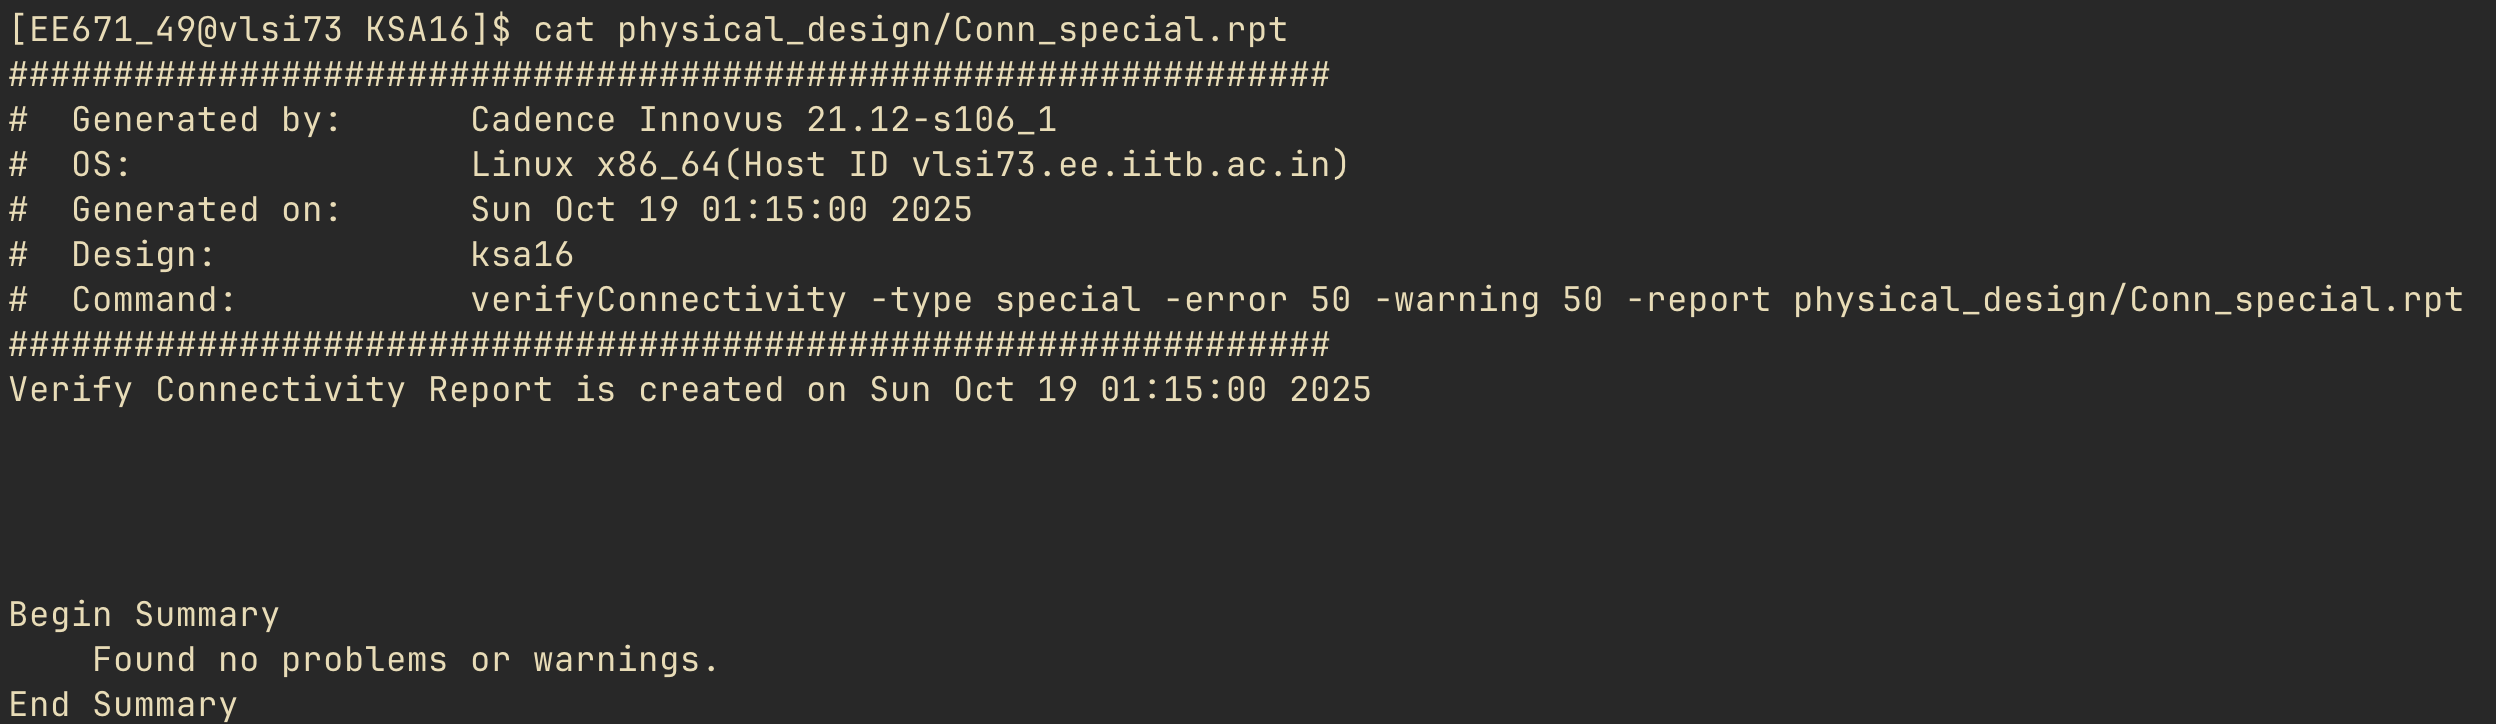
\includegraphics[width=0.95\textwidth]{conn_spc.png}
	\caption{Connectivity check for special cells}
\end{figure}

\clearpage

\section{Layout}

\begin{figure}[htbp!]
	\centering
	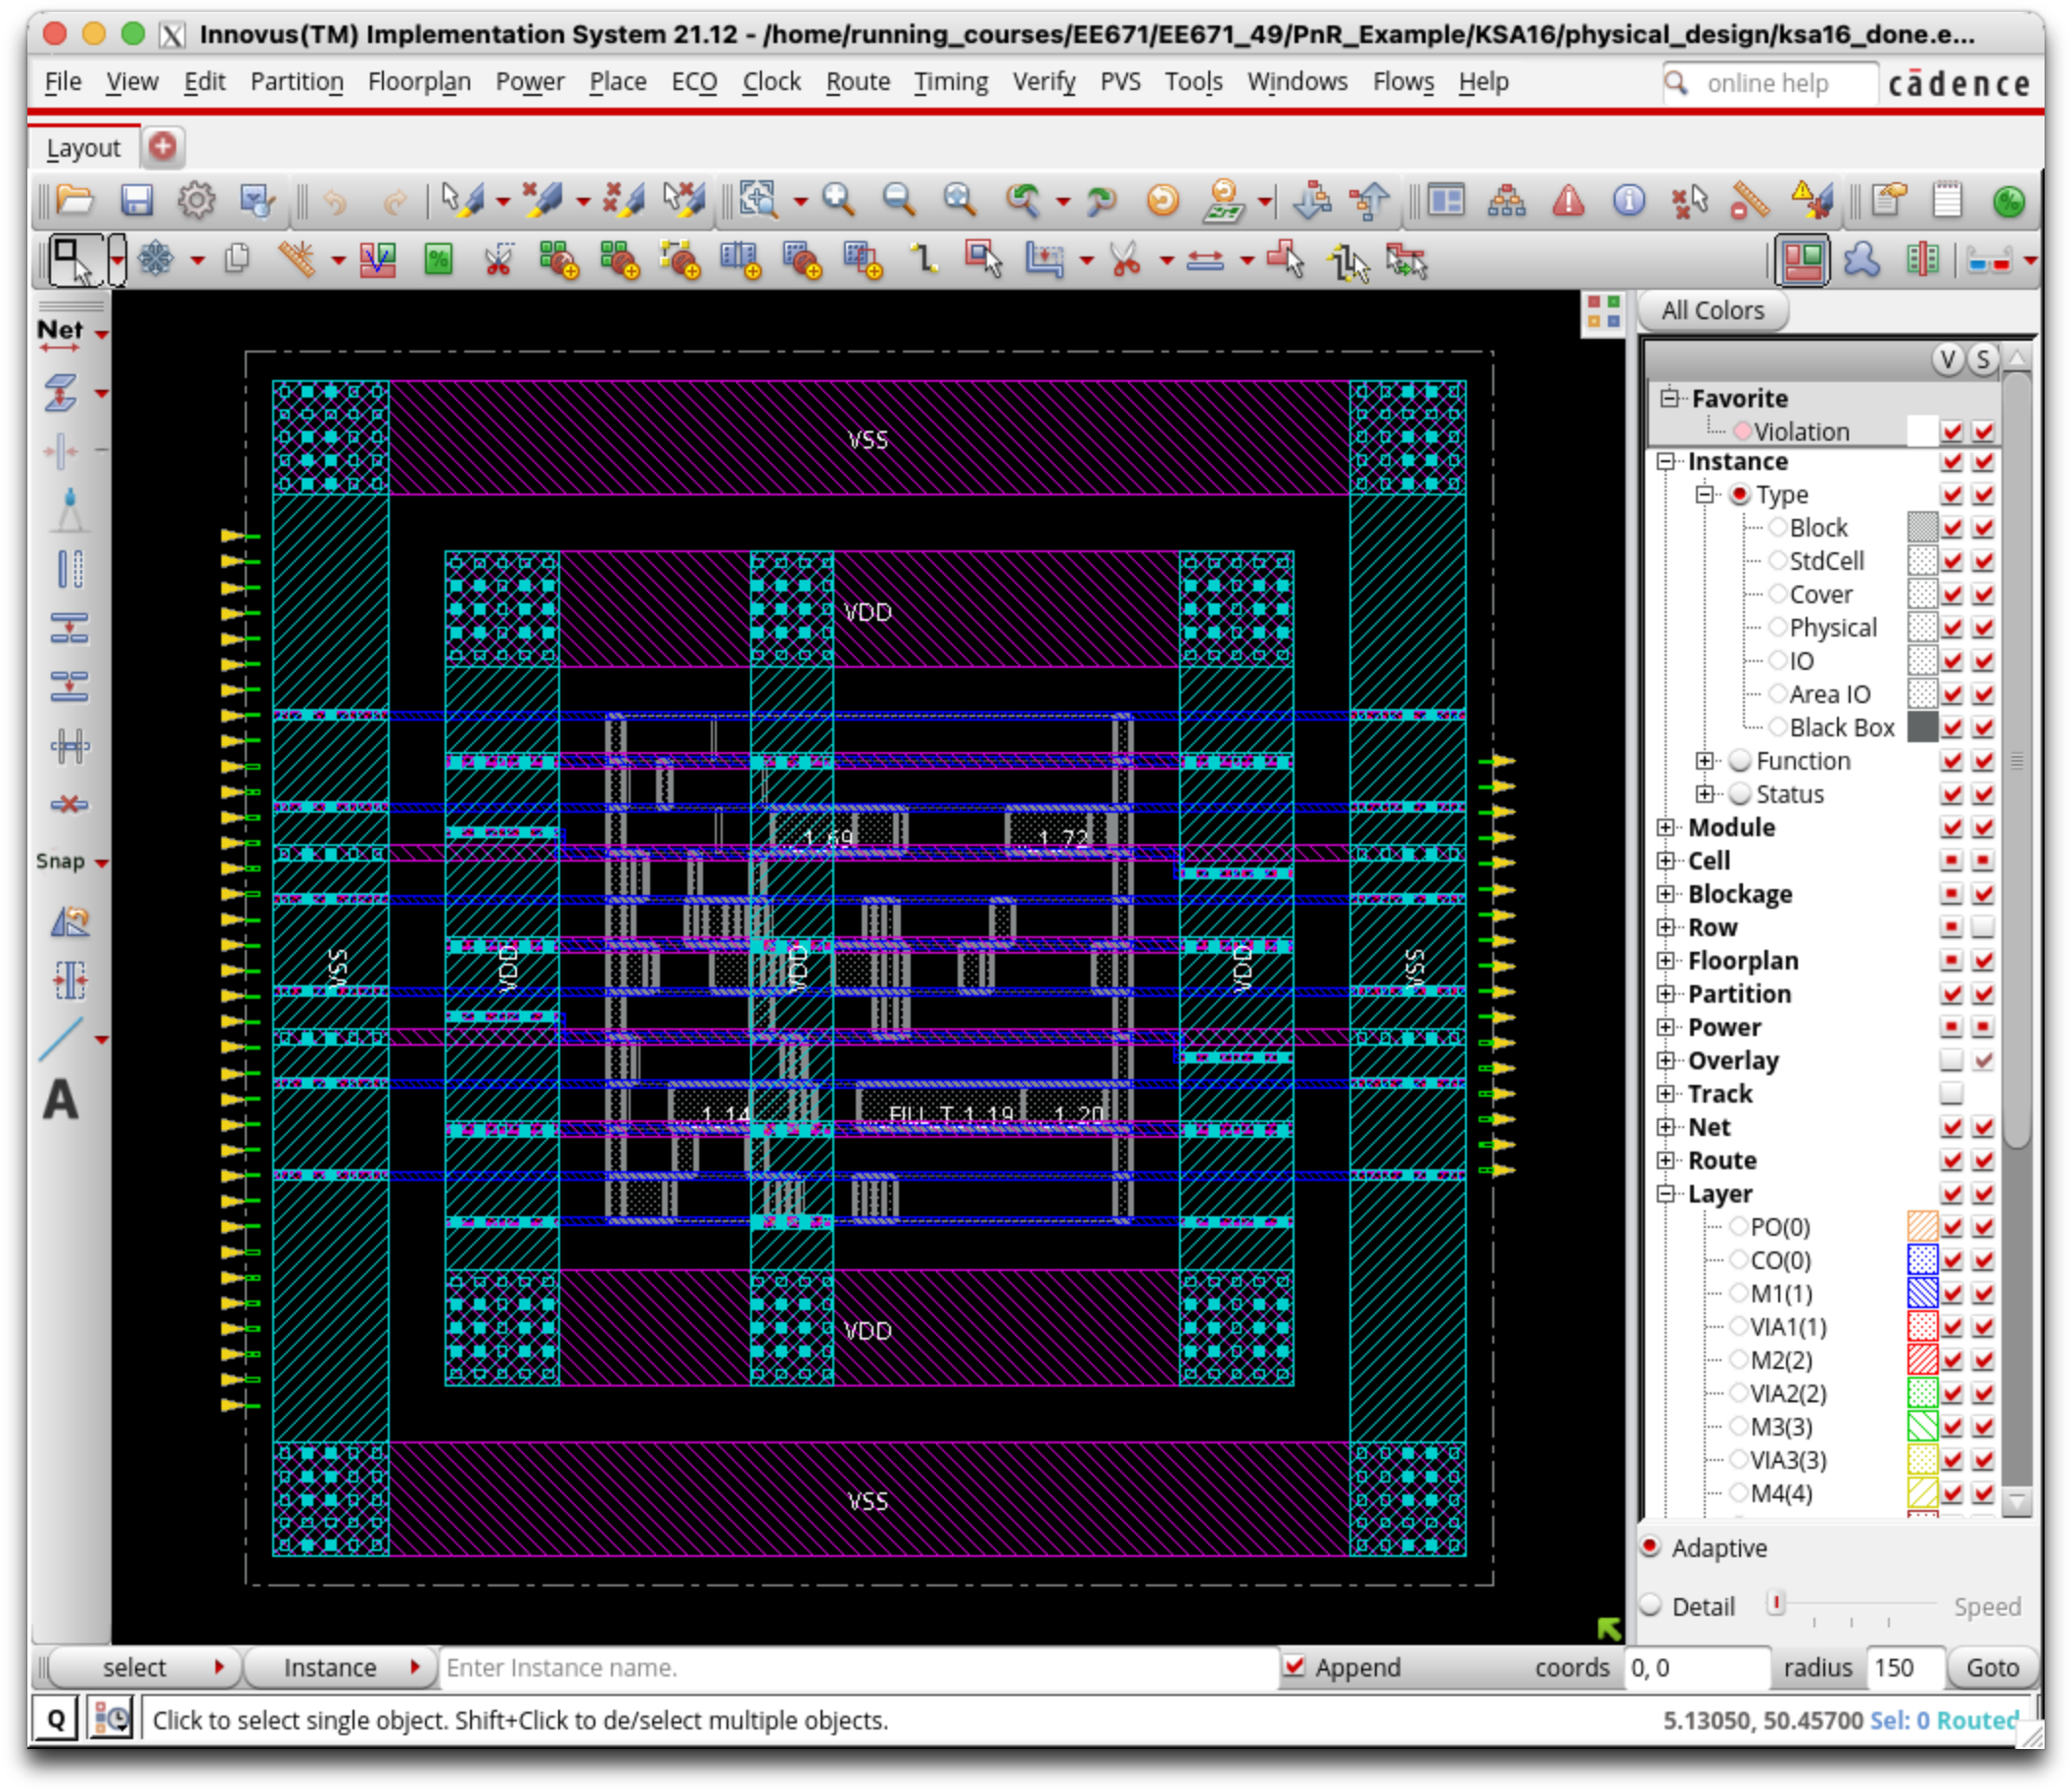
\includegraphics[width=0.95\textwidth]{layout.png}
	\caption{Post-route layout of the design}
\end{figure}

\clearpage

\section{Timing, Area and Power Analysis}

\begin{table}[htbp!]
	\centering
	\caption{Post-route Timing, Area, and Power Summary}
	\begin{tabular}{|l|l|}
		\hline
		\textbf{Parameter}                              & \textbf{Value} \\ \hline
		Clock Frequency (MHz)                           & 100            \\ \hline
		Worst Case Setup Slack [WNS] (ns)               & 8.18           \\ \hline
		Worst Case Hold Slack [WNS] (ns)                & 0.027          \\ \hline
		Design Area ($\mu$m$^2$)                        & 281.88         \\ \hline
		Power Consumption (Sequential Only) ($\mu$W)    & 27.54          \\ \hline
		Power Consumption (Combinational Only) ($\mu$W) & 12.47          \\ \hline
		Total Power (Internal Only) ($\mu$W)            & 29.54          \\ \hline
		Total Power (Switching Only) ($\mu$W)           & 2.915          \\ \hline
		Total Power (Leakage Only) ($\mu$W)             & 10.88          \\ \hline
		Total Power Consumption ($\mu$W)                & 43.34          \\ \hline
	\end{tabular}
\end{table}

\section{Post Physical Design RTL Waveform}

\begin{figure}[htbp!]
	\centering
	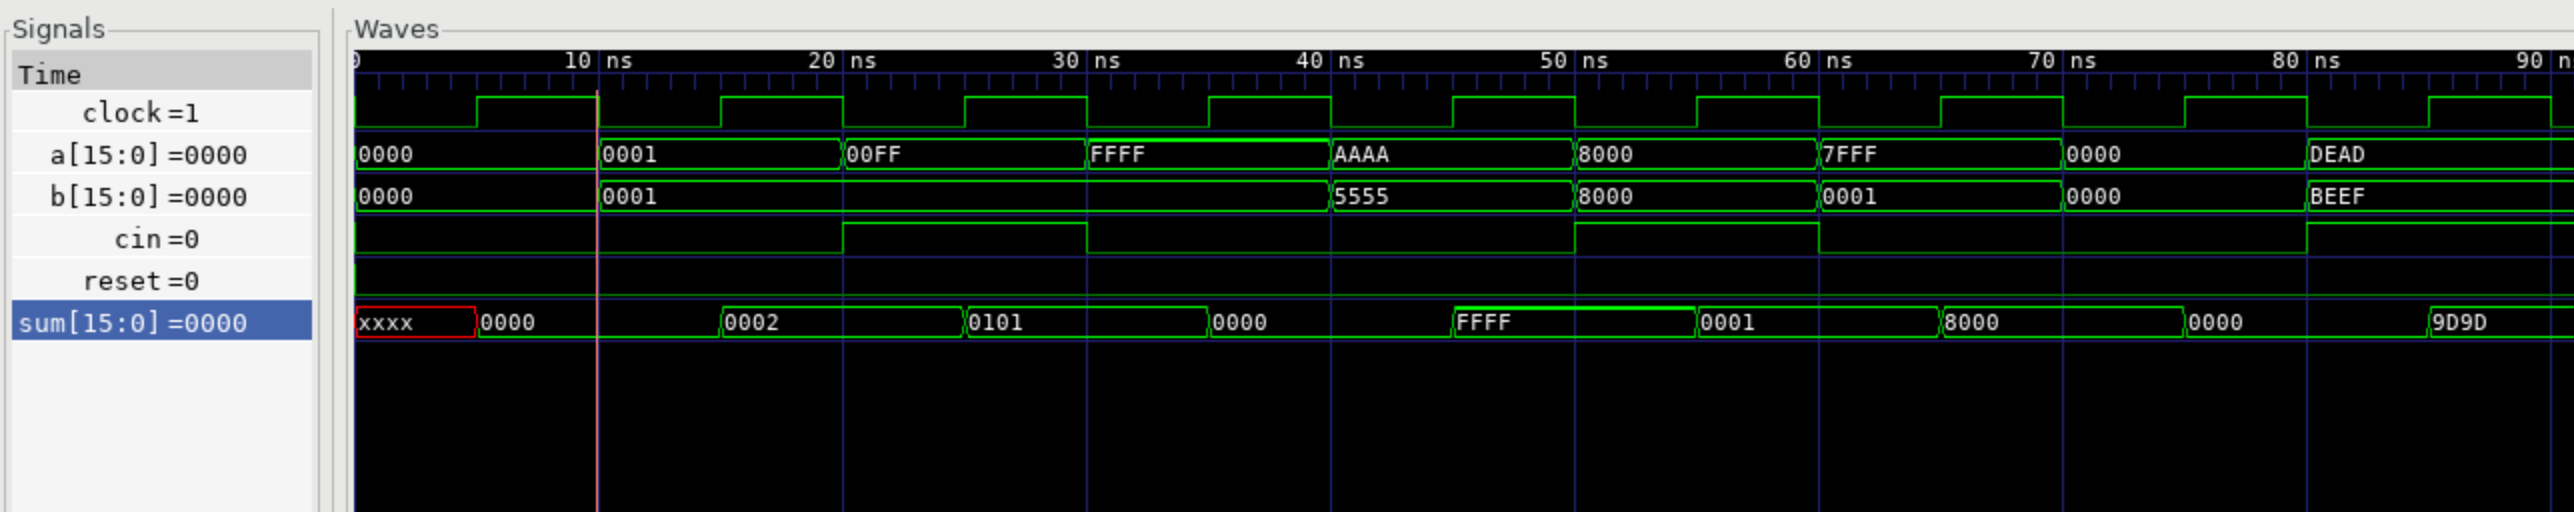
\includegraphics[width=0.95\textwidth]{post_syn.png}
	\caption{RTL waveform after physical design}
\end{figure}

\end{document}
